%%%%%%%%%%%%%%%%%%%%%%%%%%%%%%%%%%%%%%%%%
% Beamer Presentation
% LaTeX Template
% Version 1.0 (10/11/12)
%
% This template has been downloaded from:
% http://www.LaTeXTemplates.com
%
% License:
% CC BY-NC-SA 3.0 (http://creativecommons.org/licenses/by-nc-sa/3.0/)
%
%%%%%%%%%%%%%%%%%%%%%%%%%%%%%%%%%%%%%%%%%

%----------------------------------------------------------------------------------------
%	PACKAGES AND THEMES
%----------------------------------------------------------------------------------------

\documentclass{beamer}

\mode<presentation> {

	% The Beamer class comes with several default slide themes
	%, which changes the colors and layouts of slides. Below is a list
	% of all the themes, comment on each to see what they look like.

	%\usetheme{default}
	%\usetheme{AnnArbor}
	%\usetheme{Antibes}
	%\usetheme{Bergen}
	%\usetheme{Berkeley}
	%\usetheme{Berlin}
	%\usetheme{Boadilla}
	%\usetheme{CambridgeUS}
	%\usetheme{Copenhagen}
	%\usetheme{Darmstadt}
	%\usetheme{Dresden}
	%\usetheme{Frankfurt}
	%\usetheme{Goettingen}
	%\usetheme{Hannover}
	%\usetheme{Ilmenau}
	%\usetheme{JuanLesPins}
	%\usetheme{Luebeck}
	%\usetheme{Madrid}
	%\usetheme{Malmoe}
	%\usetheme{Marburg}
	%\usetheme{Montpellier}
	%\usetheme{PaloAlto}
	%\usetheme{Pittsburgh}
	\usetheme{Rochester}
	%\usetheme{Singapore}
	%\usetheme{Szeged}
	%\usetheme{Warsaw}

	% As well as themes, the Beamer class has several color themes
	% for any slide theme. Uncomment each of these, in turn, to see how it
	% changes the colors of your current slide theme.

	%\usecolortheme{albatross}
	\usecolortheme{beaver}
	%\usecolortheme{beetle}
	%\usecolortheme{crane}
	%\usecolortheme{dolphin}
	%\usecolortheme{dove}
	%\usecolortheme{fly}
	%\usecolortheme{lily}
	%\usecolortheme{orchid}
	%\usecolortheme{rose}
	%\usecolortheme{seagull}
	%\usecolortheme{seahorse}
	%\usecolortheme{whale}
	%\usecolortheme{wolverine}

	%\setbeamertemplate{footline} % To remove the footer line in all slides, uncomment this line
	%\setbeamertemplate{footline}[page number] % To replace the footer line in all slides with a simple slide count, uncomment this line

	%\setbeamertemplate{navigation symbols}{} % To remove the navigation symbols from the bottom of all slides, uncomment this line
}

\usepackage{graphicx} % Allows including images
\usepackage{booktabs} % Allows the use of \toprule, \midrule and \bottomrule in tables
% \titlegraphic{\includegraphics[height=2cm]{校徽}} % 插入校徽

\usepackage{ragged2e}
\justifying\let\raggedright\justifying %两端对齐

\usepackage{fontspec}
\setsansfont{Calibri}[
    Path=Font/,
    Scale=0.9,
    Extension = .ttf,
    UprightFont=*-Regular,
    BoldFont=*-Bold,
    ItalicFont=*-Italic,
    BoldItalicFont=*-BoldItalic
    ]
\usepackage{unicode-math}
\setmathfont{Libertinus Math} % 使用默认的数学字体或你偏好的数学字体 Latin Modern Math

\usepackage{tikz} 
%----------------------------------------------------------------------------------------
%	TITLE PAGE
%----------------------------------------------------------------------------------------

\title[Asset Pricing]{\textbf{Asset Pricing}} % The short title appears at the bottom of every slide, the full title is only on the title page

\subtitle{7. Recent Research of Asset Pricing}

\author[Cheng Hang]{Cheng Hang} % Your name
\institute[DUFE] 
{School of Fintech \\
Dongbei University of Finance \& Economics \\ 
\medskip
\textbf{chenghangch@qq.com}
}
\date{\today} 

	\AtBeginSection[]
{
	\begin{frame}{Content}
		\tableofcontents[sectionstyle=show/shaded,subsectionstyle=show/shaded/hide] %这几个参数我也不知道该如何准确地解释，反正它们最终的效果是突出显示当前章节，而其它章节都进行了淡化处理
		\addtocounter{framenumber}{-1}  %目录页不计算页码
	\end{frame}
}

%----------------------------------------------------------------------------------------
%	Begin
%----------------------------------------------------------------------------------------

\begin{document}

\begin{frame}
\titlepage % Print the title page as the first slide
\end{frame}

%----------------------------------------------------------------------------------------
%	PRESENTATION SLIDES
%----------------------------------------------------------------------------------------


% Section 1
\section{Motivation}

\begin{frame}{The Puzzle: Time-Series vs. Cross-Section}
\begin{itemize}
\item \textbf{Empirical observation:} Many variables predict aggregate market returns in time-series
\begin{itemize}
\item Dividend yield, term spread, default spread, market volatility
\item Valuation ratios, macroeconomic indicators
\end{itemize}
\vspace{0.3cm}
\item \textbf{The question:} Should time-series predictors also matter for cross-sectional pricing?
\vspace{0.3cm}
\item \textbf{Our answer:} Yes, under the ICAPM framework
\begin{itemize}
\item Time-series predictability signals changes in investment opportunities
\item Shocks to these variables represent systematic risks
\item Cross-sectional risk premia compensate for exposure to these shocks
\end{itemize}
\end{itemize}
\end{frame}

\begin{frame}{Research Questions}
\begin{enumerate}
\item What is the theoretical link between time-series predictability and cross-sectional pricing?
\vspace{0.3cm}
\item How can we empirically test this dual implication?
\vspace{0.3cm}
\item What does this framework tell us about the nature of risk factors?
\end{enumerate}
\end{frame}

% Section 2
\section{Theoretical Framework}

\begin{frame}{Merton's ICAPM (1973)}
\textbf{Key insight:} Investors care about two types of risks
\begin{enumerate}
\item \textbf{Market risk:} Variation in current wealth
\item \textbf{Intertemporal risk:} Changes in future investment opportunities
\end{enumerate}

\vspace{0.5cm}
\textbf{Pricing equation:}
$$E[r_i] - r_f = \beta_i^m \lambda^m + \sum_{j=1}^{K} \beta_i^{z_j} \lambda^{z_j}$$

where:
\begin{itemize}
\item $\beta_i^m$: exposure to market portfolio
\item $\beta_i^{z_j}$: exposure to state variable $z_j$ innovations
\item $\lambda^{z_j}$: risk premium for state variable $j$
\end{itemize}
\end{frame}

\begin{frame}{State Variables in ICAPM}
\textbf{Definition:} A state variable $z_t$ captures shifts in investment opportunities if:
\begin{enumerate}
\item It predicts future market returns or investment opportunities
\item Its innovations cannot be diversified away
\item Investors demand compensation for exposure to its shocks
\end{enumerate}

\vspace{0.5cm}
\textbf{Examples:}
\begin{itemize}
\item Variables affecting expected returns: dividend yield, term spread
\item Variables affecting return volatility: VIX, realized volatility
\item Variables affecting consumption/wealth: GDP growth, unemployment
\end{itemize}
\end{frame}

% Section 3
\section{Time-Series Dimension}

\begin{frame}{Time-Series Predictability}
\textbf{Predictive regression:}
$$r_{m,t+1} = a + b \cdot z_t + \varepsilon_{t+1}$$

\vspace{0.3cm}
\textbf{Interpretation:}
\begin{itemize}
\item If $b \neq 0$ (statistically significant), then $z_t$ predicts market returns
\item Predictability suggests time-variation in expected returns
\item $z_t$ contains information about future investment opportunities
\end{itemize}

\vspace{0.3cm}
\textbf{Economic mechanism:}
\begin{itemize}
\item High $z_t$ may signal higher future expected returns (compensation for risk)
\item Or lower future expected returns (good investment opportunities)
\item Direction depends on the economic nature of $z_t$
\end{itemize}
\end{frame}

\begin{frame}{Extracting Innovations}
\textbf{Challenge:} We need \textit{unexpected} changes in $z_t$, not predictable movements

\vspace{0.3cm}
\textbf{Method:} Model the dynamics of $z_t$
$$z_{t+1} = \alpha + \rho \cdot z_t + u_{t+1}$$

\vspace{0.3cm}
\textbf{Innovation:}
$$\Delta z_{t+1}^{innov} = z_{t+1} - E_t[z_{t+1}] = z_{t+1} - (\alpha + \rho \cdot z_t) = u_{t+1}$$

\vspace{0.3cm}
\textbf{Key property:} $\Delta z_{t+1}^{innov}$ is orthogonal to information at time $t$
\begin{itemize}
\item Represents true surprises to investors
\item Cannot be hedged using time-$t$ information
\end{itemize}
\end{frame}

% Section 4
\section{Cross-Sectional Dimension}

\begin{frame}{Cross-Sectional Risk Exposure}
\textbf{Factor loading:} Measure each asset's sensitivity to state variable shocks
$$\beta_i^z = \frac{\text{Cov}(r_i, \Delta z^{innov})}{\text{Var}(\Delta z^{innov})}$$

\vspace{0.3cm}
\textbf{Interpretation:}
\begin{itemize}
\item $\beta_i^z > 0$: Asset $i$ pays off when $z$ increases unexpectedly
\item $\beta_i^z < 0$: Asset $i$ pays off when $z$ decreases unexpectedly
\item $\beta_i^z = 0$: Asset $i$ is unrelated to $z$ shocks
\end{itemize}

\vspace{0.3cm}
\textbf{Economic intuition:}
\begin{itemize}
\item Assets with different $\beta_i^z$ provide different hedging properties
\item Investors value assets that hedge against adverse shocks
\end{itemize}
\end{frame}

\begin{frame}{Cross-Sectional Pricing}
\textbf{ICAPM prediction:} Expected returns should be linearly related to $\beta_i^z$
$$E[r_i] - r_f = \beta_i^m \lambda^m + \beta_i^z \lambda^z$$

\vspace{0.3cm}
\textbf{Price of risk $\lambda^z$:}
\begin{itemize}
\item $\lambda^z > 0$: Assets with higher $\beta_i^z$ earn higher returns
\item $\lambda^z < 0$: Assets with higher $\beta_i^z$ earn lower returns
\item Sign depends on whether shocks to $z$ are "good" or "bad" for investors
\end{itemize}

\vspace{0.3cm}
\textbf{Example:}
\begin{itemize}
\item If positive shocks to volatility ($z$ = VIX) worsen investment opportunities
\item Then $\lambda^z > 0$ (compensation for volatility risk)
\item Assets with $\beta_i^z > 0$ (increase when volatility rises) earn higher returns
\end{itemize}
\end{frame}

% Section 5
\section{The Linkage}

\begin{frame}{Time-Series $\Leftrightarrow$ Cross-Section}
\begin{center}
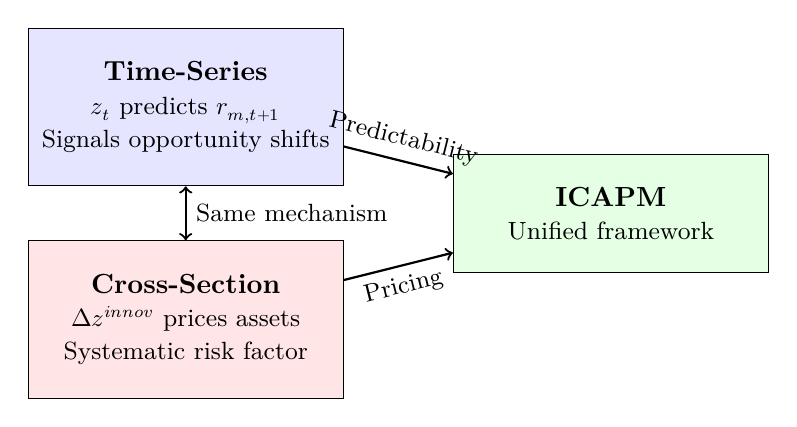
\begin{tikzpicture}[scale=0.9]
% Time-series box
\node[draw, rectangle, minimum width=4cm, minimum height=2cm, align=center, fill=blue!10] (ts) at (0,3) 
{{\bf Time-Series} \\ \small $z_t$ predicts $r_{m,t+1}$ \\ \small Signals opportunity shifts};

% Cross-section box
\node[draw, rectangle, minimum width=4cm, minimum height=2cm, align=center, fill=red!10] (cs) at (0,0) 
{{\bf Cross-Section} \\ \small $\Delta z^{innov}$ prices assets \\ \small Systematic risk factor};

% ICAPM box
\node[draw, rectangle, minimum width=4cm, minimum height=1.5cm, align=center, fill=green!10] (icapm) at (6,1.5) 
{{\bf ICAPM} \\ \small Unified framework};

% Arrows
\draw[->, thick] (ts) -- (icapm) node[midway, above, sloped] {\small Predictability};
\draw[->, thick] (cs) -- (icapm) node[midway, below, sloped] {\small Pricing};
\draw[<->, thick] (ts) -- (cs) node[midway, right] {\small Same mechanism};
\end{tikzpicture}
\end{center}

\vspace{0.3cm}
\textbf{Key insight:} Two sides of the same coin
\begin{itemize}
\item Time-series: $z_t$ forecasts aggregate opportunities
\item Cross-section: $\Delta z^{innov}$ represents systematic risk
\end{itemize}
\end{frame}

\begin{frame}{Economic Mechanism}
\begin{enumerate}
\item \textbf{State variable dynamics:}
\begin{itemize}
\item $z_t$ evolves over time, capturing shifts in investment opportunities
\item Investors observe $z_t$ and update expectations
\end{itemize}
\vspace{0.2cm}

\item \textbf{Time-series manifestation:}
\begin{itemize}
\item Changes in $z_t$ predict changes in aggregate market returns
\item Reflects time-varying risk premia or expected returns
\end{itemize}
\vspace{0.2cm}

\item \textbf{Cross-sectional manifestation:}
\begin{itemize}
\item Unexpected shocks to $z_t$ affect assets differentially
\item Assets with higher exposure to these shocks require higher returns
\end{itemize}
\vspace{0.2cm}

\item \textbf{Risk-return tradeoff:}
\begin{itemize}
\item Investors demand compensation for bearing exposure to $\Delta z^{innov}$
\item Assets that hedge against adverse shocks earn lower returns
\end{itemize}
\end{enumerate}
\end{frame}

\begin{frame}{Why Both Tests Matter}
\textbf{Time-series test alone is insufficient:}
\begin{itemize}
\item Many variables predict returns due to data mining
\item Predictability does not guarantee it is a priced risk factor
\item May reflect market inefficiency or other mechanisms
\end{itemize}

\vspace{0.3cm}
\textbf{Cross-sectional test alone is insufficient:}
\begin{itemize}
\item Factor may price assets but lack economic interpretation
\item Difficult to distinguish systematic risk from characteristics
\item No clear link to investment opportunity changes
\end{itemize}

\vspace{0.3cm}
\textbf{Combined tests provide strong evidence:}
\begin{itemize}
\item Validates ICAPM theory: state variables matter in both dimensions
\item Rules out spurious factors and data mining
\item Identifies genuine risks affecting investment opportunities
\end{itemize}
\end{frame}

% Section 6
\section{Empirical Implementation}

\begin{frame}{Four-Step Procedure}
\textbf{Step 1: Time-series predictability}
$$r_{m,t+1} = a + b \cdot z_t + \varepsilon_{t+1}$$
Test $H_0: b = 0$ using Newey-West standard errors

\vspace{0.3cm}
\textbf{Step 2: Extract innovations}
\begin{itemize}
\item Estimate AR(1) or VAR model for $z_t$
\item Compute $\Delta z_{t+1}^{innov} = z_{t+1} - E_t[z_{t+1}]$
\end{itemize}

\vspace{0.3cm}
\textbf{Step 3: Estimate factor loadings}
\begin{itemize}
\item Regress individual returns on $r_m$ and $\Delta z^{innov}$
\item Obtain $\hat{\beta}_i^z$ for each asset $i$
\end{itemize}

\vspace{0.3cm}
\textbf{Step 4: Test cross-sectional pricing}
\begin{itemize}
\item Fama-MacBeth regressions or GMM estimation
\item Test $H_0: \lambda^z = 0$
\end{itemize}
\end{frame}

\begin{frame}{Portfolio Sorting Approach}
\textbf{Alternative method:} Sort assets into portfolios based on $\beta_i^z$

\vspace{0.3cm}
\textbf{Procedure:}
\begin{enumerate}
\item Estimate $\beta_i^z$ for each asset using rolling windows
\item Sort assets into deciles based on $\beta_i^z$
\item Construct equal-weighted or value-weighted portfolios
\item Compute average returns for each decile
\end{enumerate}

\vspace{0.3cm}
\textbf{Expected pattern (if $\lambda^z > 0$):}
\begin{itemize}
\item Portfolio 1 (low $\beta^z$): Low average return
\item Portfolio 10 (high $\beta^z$): High average return
\item Monotonic increase across deciles
\end{itemize}

\vspace{0.3cm}
\textbf{Statistical tests:}
\begin{itemize}
\item Test whether high-minus-low portfolio return is significant
\item Examine whether spread persists after controlling for other factors
\end{itemize}
\end{frame}

\begin{frame}{Robustness Checks}
\textbf{Address potential concerns:}

\begin{enumerate}
\item \textbf{Endogeneity and reverse causality}
\begin{itemize}
\item Use instrumental variables for $z_t$ in predictive regressions
\item Lag $z_t$ by multiple periods
\end{itemize}
\vspace{0.2cm}

\item \textbf{Overlapping observations}
\begin{itemize}
\item Use Newey-West or Hansen-Hodrick standard errors
\item Consider alternative forecast horizons
\end{itemize}
\vspace{0.2cm}

\item \textbf{Factor model specification}
\begin{itemize}
\item Control for Fama-French factors, momentum, liquidity
\item Test incremental explanatory power of $\Delta z^{innov}$
\end{itemize}
\vspace{0.2cm}

\item \textbf{Sample period and data frequency}
\begin{itemize}
\item Examine sub-period stability
\item Test at different frequencies (daily, monthly, quarterly)
\end{itemize}
\end{enumerate}
\end{frame}

% Section 7
\section{Economic Interpretation}

\begin{frame}{What Makes a Valid State Variable?}
\textbf{Three conditions must hold:}

\begin{enumerate}
\item \textbf{Time-series predictability}
\begin{itemize}
\item $z_t$ forecasts future market returns or volatility
\item Evidence that $z_t$ captures investment opportunity shifts
\end{itemize}
\vspace{0.2cm}

\item \textbf{Systematic risk}
\begin{itemize}
\item Innovations to $z_t$ cannot be diversified away
\item Shocks to $z_t$ affect broad set of assets
\end{itemize}
\vspace{0.2cm}

\item \textbf{Cross-sectional pricing}
\begin{itemize}
\item Assets with different exposures to $\Delta z^{innov}$ earn different returns
\item Risk premium $\lambda^z$ is economically and statistically significant
\end{itemize}
\end{enumerate}

\vspace{0.3cm}
\textbf{Variables satisfying all three conditions are genuine ICAPM state variables}
\end{frame}

\begin{frame}{Examples from the Literature}
\begin{table}
\centering
\small
\begin{tabular}{lll}
\toprule
\textbf{State Variable} & \textbf{Time-Series} & \textbf{Cross-Section} \\
\midrule
Dividend yield & Predicts returns & Dividend growth risk \\
Term spread & Predicts returns & Interest rate risk \\
Default spread & Predicts returns & Credit risk \\
VIX & Predicts volatility & Volatility risk \\
Aggregate volatility & Predicts returns & Volatility risk \\
Labor income growth & Predicts consumption & Human capital risk \\
\bottomrule
\end{tabular}
\end{table}

\vspace{0.3cm}
\textbf{Key papers:}
\begin{itemize}
\item Campbell (1996): Dividend yield and intertemporal substitution
\item Fama and French (1989): Term and default spreads
\item Ang et al. (2006): Aggregate volatility risk
\end{itemize}
\end{frame}

\begin{frame}{Hedging Interpretation}
\textbf{Assets as hedging instruments:}

\vspace{0.3cm}
Consider two assets with different $\beta^z$:
\begin{itemize}
\item \textbf{Asset A:} $\beta_A^z = 1.5$ (amplifies shocks to $z$)
\item \textbf{Asset B:} $\beta_B^z = -0.5$ (hedges shocks to $z$)
\end{itemize}

\vspace{0.3cm}
If positive shocks to $z$ worsen investment opportunities ($\lambda^z > 0$):
\begin{itemize}
\item Asset A is risky: pays off when opportunities are already good
\item Asset B is a hedge: pays off when opportunities deteriorate
\item Therefore, $E[r_A] > E[r_B]$ in equilibrium
\end{itemize}

\vspace{0.3cm}
\textbf{Intuition:} Investors pay a premium (accept lower returns) for assets that hedge against adverse shifts in investment opportunities
\end{frame}

% Section 8
\section{Application to Chinese A-Share Market}

\begin{frame}{Potential State Variables for China}
\textbf{Macroeconomic variables:}
\begin{itemize}
\item Industrial production growth
\item M2 money supply growth
\item Credit growth and social financing
\item PMI (Purchasing Managers' Index)
\end{itemize}

\vspace{0.3cm}
\textbf{Market-based variables:}
\begin{itemize}
\item Aggregate turnover and liquidity measures
\item Market volatility (realized or implied)
\item Valuation ratios (P/E, P/B at market level)
\item Investor sentiment indices
\end{itemize}

\vspace{0.3cm}
\textbf{Policy-related variables:}
\begin{itemize}
\item Monetary policy shocks
\item Regulatory policy uncertainty
\item Government intervention intensity
\end{itemize}
\end{frame}

\begin{frame}{Institutional Features of A-Share Market}
\textbf{Considerations for empirical implementation:}

\begin{enumerate}
\item \textbf{Short-selling constraints}
\begin{itemize}
\item Limits arbitrage and price efficiency
\item May amplify or dampen certain risk premia
\end{itemize}
\vspace{0.2cm}

\item \textbf{Retail investor dominance}
\begin{itemize}
\item Higher sentiment-driven volatility
\item State variables related to sentiment may be more relevant
\end{itemize}
\vspace{0.2cm}

\item \textbf{Government intervention}
\begin{itemize}
\item Policy shocks as state variables
\item Time-varying effectiveness of traditional factors
\end{itemize}
\vspace{0.2cm}

\item \textbf{Market segmentation}
\begin{itemize}
\item Different dynamics for SOEs vs. private firms
\item Regional and sector-specific factors
\end{itemize}
\end{enumerate}
\end{frame}

% Section 9
\section{Conclusion}

\begin{frame}{Summary}
\textbf{Main contributions:}

\begin{enumerate}
\item \textbf{Theoretical linkage:} ICAPM provides unified framework
\begin{itemize}
\item Time-series predictability and cross-sectional pricing are connected
\item Both reflect the same economic mechanism: state variable dynamics
\end{itemize}
\vspace{0.2cm}

\item \textbf{Empirical discipline:} Dual testing requirements
\begin{itemize}
\item Rules out spurious factors from data mining
\item Identifies genuine state variables affecting investment opportunities
\end{itemize}
\vspace{0.2cm}

\item \textbf{Economic interpretation:} Risk vs. hedging
\begin{itemize}
\item High $\beta^z$ assets bear risk, earn high returns
\item Low $\beta^z$ assets provide hedging, earn low returns
\end{itemize}
\end{enumerate}

\vspace{0.3cm}
\textbf{Key insight:} Variables that pass both tests are economically meaningful state variables in the ICAPM sense
\end{frame}

\begin{frame}{Implications for Asset Pricing Research}
\textbf{Research strategy:}

\begin{enumerate}
\item Start with economic theory to identify candidate state variables
\vspace{0.2cm}

\item Test time-series predictability to validate opportunity shifts
\vspace{0.2cm}

\item Construct innovation series and test cross-sectional pricing
\vspace{0.2cm}

\item Interpret results through ICAPM lens (risk vs. hedging)
\vspace{0.2cm}

\item Examine robustness and economic magnitudes
\end{enumerate}

\vspace{0.3cm}
\textbf{Advantages:}
\begin{itemize}
\item Strong theoretical foundation (Merton 1973)
\item Clear empirical predictions
\item Economically interpretable results
\item Distinguishes systematic risks from spurious factors
\end{itemize}
\end{frame}

\begin{frame}{Future Research Directions}
\begin{enumerate}
\item \textbf{International comparison}
\begin{itemize}
\item Which state variables are universal vs. market-specific?
\item How do institutional features affect pricing?
\end{itemize}
\vspace{0.2cm}

\item \textbf{Time-varying risk premia}
\begin{itemize}
\item Does $\lambda^z$ vary over time?
\item What drives variation in risk premia?
\end{itemize}
\vspace{0.2cm}

\item \textbf{Higher moments}
\begin{itemize}
\item Do innovations in skewness and kurtosis matter?
\item Non-linear relationships between $\beta^z$ and returns
\end{itemize}
\vspace{0.2cm}

\item \textbf{Machine learning applications}
\begin{itemize}
\item Identify state variables using ML techniques
\item Non-parametric estimation of pricing kernels
\end{itemize}
\end{enumerate}
\end{frame}

\begin{frame}[c]
\begin{center}
{\Large Thank You!}

\vspace{1cm}

{\large Questions and Discussion}
\end{center}
\end{frame}

% References
\begin{frame}[allowframebreaks]{References}
\small
\begin{itemize}
\item Merton, R. C. (1973). An intertemporal capital asset pricing model. \textit{Econometrica}, 41(5), 867-887.
\vspace{0.2cm}

\item Campbell, J. Y. (1996). Understanding risk and return. \textit{Journal of Political Economy}, 104(2), 298-345.
\vspace{0.2cm}

\item Fama, E. F., \& French, K. R. (1989). Business conditions and expected returns on stocks and bonds. \textit{Journal of Financial Economics}, 25(1), 23-49.
\vspace{0.2cm}

\item Ang, A., Hodrick, R. J., Xing, Y., \& Zhang, X. (2006). The cross-section of volatility and expected returns. \textit{Journal of Finance}, 61(1), 259-299.
\vspace{0.2cm}

\item Cochrane, J. H. (2011). Presidential address: Discount rates. \textit{Journal of Finance}, 66(4), 1047-1108.
\vspace{0.2cm}

\item Campbell, J. Y., \& Vuolteenaho, T. (2004). Bad beta, good beta. \textit{American Economic Review}, 94(5), 1249-1275.
\end{itemize}
\end{frame}

\end{document}
